\subsection{ResNet介绍}

\begin{wrapfigure}{r}{0.3\textwidth}
    \centering %表示居中
    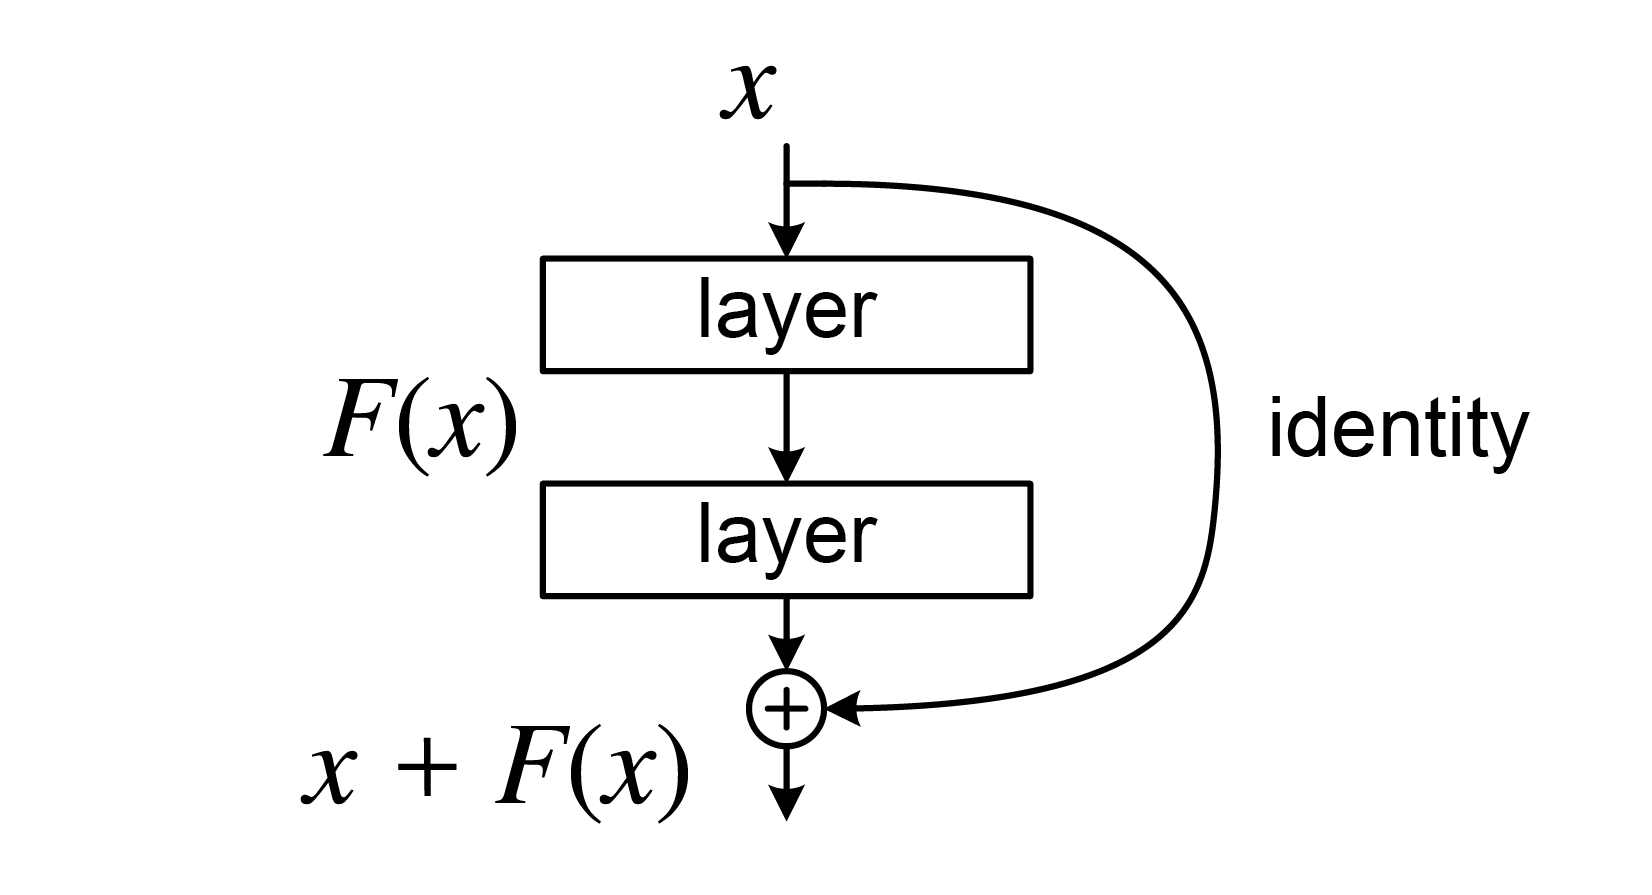
\includegraphics[height=2.5cm]{../../ResNet/ResBlock.png}
    \caption{ResNet中残差块的结构}
\end{wrapfigure}

ResNet是一个划时代的深度神经网络架构,它是由Kaiming He,Xiangyu Zhang,Shaoqing Ren,Jian Sun于2015年提出的。\cite{ResNet}
残差学习是利用残差块的设计,实现前层特征的直接传递。
这样的结构成功地解决了随着网络加深,梯度会逐渐消失的问题。
这使得ResNet可以使用很深的神经网络进行训练。
ResNet-152层的网络在ImageNet图像分类任务上取得了3.57\%的top-5的错误率,对当时视觉领域造成了巨大的影响。 \par

总的来说,ResNet开创了深度残差网络的新范式。
它简单而高效的架构设计,成功地训练了百层级甚至千层级的超深网络,使得超深的神经网络成为现实。
同时,ResNet在识别的过程中也有着很高的成功率,是图像识别神经网络的一个重要选择。

\subsection{使用ResNet对图像进行识别的效果分析}
训练结果如下:
\begin{table}[H]
    \begin{minipage}[b]{0.56\linewidth}
    \centering
    \begin{tabular}{c|c|c}
        \hline
        Epoch & Loss & Test Accuracy \\ \hline \hline
        10 & 0.92 & 67.15 \\ \hline
        20 & 0.70 & 67.97 \\ \hline
        30 & 0.57 & 79.67 \\ \hline
        40 & 0.47 & 78.44 \\ \hline
        50 & 0.40 & 86.24 \\ \hline
       \end{tabular}
        \caption{随训练轮数增加Loss和Test Accuracy的变化}
    \end{minipage}
    \begin{minipage}[b]{0.4\linewidth}
    \centering
    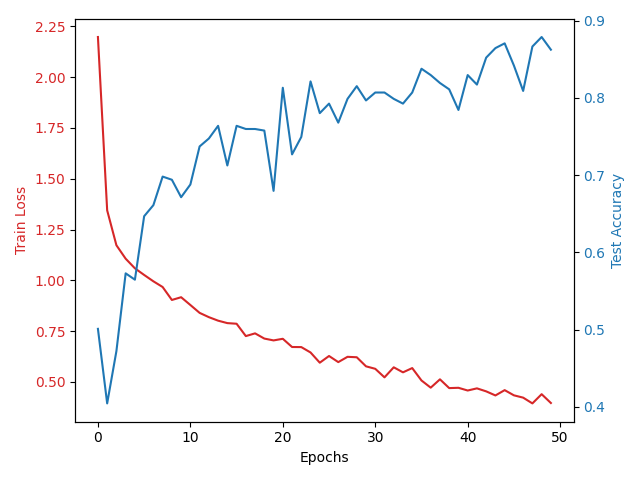
\includegraphics[width=50mm]{../../ResNet/ResNet.png}
    \captionof{figure}{ResNet训练结果}
    \end{minipage}
    \end{table}

通过分析识别的准确率可以发现,使用ResNet进行训练,随着训练的轮数增加,Loss逐渐下降,而准确率不断上升。
在训练45轮左右时,准确率基本稳定在85\%左右,且仍有上升势头。
发现在50轮训练的过程中并未出现过拟合的现象,原因可能是ResNet的网络深度比较深,较少轮数的训练不足以达到过拟合的情况。 \par
总的来说,ResNet识别的准确率相较于AlexNet高出近20\%,具有长足提升。
这可能得益于其具有的更深的神经网络和残差块的结构。
